\section{Auswirkungen einer SOA auf den Auslieferungsprozess}
\label{ch:deliveryProcess}
Auslieferung von Software beschreibt den Prozess der Verteilung, Installation beziehungsweise Aktualisierung und Konfiguration von Software für den produktiven Einsatz. Üblicherweise werden hierbei Softwarepakete mit zugehörigen Nutzungsrechten vom Softwarehersteller an den Softwarebetreiber übertragen.\\
Dabei existieren völlig unterschiedliche Herangehensweisen für den Auslieferungsprozess. Je nach Art der auszuliefernden Software und dem späteren Einsatz kann entweder manuell oder automatisiert ausgeliefert werden. Dabei existieren unzählige Zwischenstufen mit unterschiedlichen Automatisierungsgraden. Des Weiteren kann Software beispielsweise entweder über ein Netzwerk oder über ein physisches Installationsmedium ausgeliefert werden. Auch die Art und Frequenz der Durchführung von Aktualisierungen kann sich erheblich unterscheiden. Darüber hinaus existieren viele weitere Möglichkeiten und Eigenschaften, in welchen sich der Auslieferungsprozess eines Softwaresystems unterscheiden kann.\\
Viele der Entscheidungen für die Gestaltung des Auslieferungsprozesses hängen weniger von der Architektur der Software ab als viel mehr von der Art des Systems und von den Wünschen des Kunden. Daher werden viele mögliche Eigenschaften des Auslieferungsprozesses in diesem Abschnitt nicht behandelt. Dennoch ergeben sich aus der Wahl der Softwarearchitektur unterschiedliche Möglichkeiten beziehungsweise Vor- und Nachteile, welche insbesondere bei der Wahl der Verteilungsstrategie ausschlaggebend sind. Einige Verteilungsstrategien werden im nächsten Abschnitt vorgestellt.

Eine wesentliche Eigenschaft von Services ist ihre Eigenständigkeit und Unabhängigkeit. Um diese Eigenschaften auch im Prozess der Auslieferung von serviceorientierten Systemen in größtmöglichem Umfang beibehalten zu können, werden Services üblicherweise in virtuellen Maschinen (VMs) gekapselt und ausgeliefert. VMs sind komplexe Softwaresysteme, die eine isolierte Umgebung auf einem Rechnersystem darstellen. Sie emulieren physische Maschinen und stellen eine Umgebung bereit, welche exakt wie die physische Maschine reagiert, unabhängig von dem tatsächlichen physischen System auf welchem die VM läuft.\\
Der große Vorteil von Virtualisierung ist, dass jegliche Software innerhalb einer VM zunächst vollständig vom außenstehenden System isoliert ist. Zum einen ist ein Service somit von unerwünschtem Zugriff von außen geschützt, da Zugriffsmöglichkeiten zunächst explizit freigegeben werden müssen. Zum anderen ist die Software innerhalb der VM völlig unabhängig von dem physischen System, auf welchem diese läuft, sodass die Software mitsamt der VM auf einen beliebigen anderen virtualisierten Host portiert werden kann. Somit ist ein Service nicht nur positionsunabhängig adressierbar, sondern auch positionsunabhängig ausführbar.\\
Für Microservices werden außerdem oftmals Container für die Kapselung genutzt. Diese haben den Vorteil, dass sie wesentlich leichtgewichtiger sind und somit in sehr dynamischen Systemen eine schnellere Skalierung mit weniger Overhead ermöglichen. Jedoch ist die Software innerhalb eines Containers nicht vollständig isoliert, da beispielsweise mehrere Container auf einem Host denselben Kernel nutzen. Daraus resultieren erhebliche Einbußen hinsichtlich der Sicherheit und Isoliertheit eines serviceorientierten Systems, da sich Software, die in separaten Containern jedoch auf demselben Host läuft, gegenseitig über den Host-Kernel korrumpieren kann.\\
In beiden Fällen wird jedoch eine Kapselung der verwendeten Technologie erreicht, sodass für die Auslieferung und Inbetriebnahme lediglich die API der Virtualisierungs- beziehungsweise Containerisierungslösung bekannt sein muss. Es wird kein weiteres Wissen hinsichtlich der Technologie des Services benötigt. Die Vorteile im Auslieferungsprozess werden allerdings mit erhöhter Komplexität beim Bauprozess aufgewogen, da hier zusätzlich die Images für die VMs oder Container erstellt werden müssen.\\
Die Verwendung einer SOA und die gewonnene Flexibilität durch die daraus resultierende lose Kopplung ermöglicht zusätzlich eine wesentlich agilere Auslieferung von Aktualisierungen und flexiblere Möglichkeiten für die Skalierung eines Softwaresystems.\\
Im Folgenden werden diese Möglichkeiten genauer erläutert.

\subsection{Skalierung}
\label{sec:scaling}
Ein System, bestehend aus autonomen Services kann sowohl horizontal als auch vertikal unproportional skaliert werden. Unproportionale Skalierung meint hierbei, dass einzelne Services des Systems in beliebige Richtung skaliert werden können, während andere Services ihre Kapazität halten. Somit kann sich das Gesamtsystem dynamisch an beliebige Lastszenarien anpassen \cite{NADAREISHVILI.2016}.\\
Weitere oder leistungsfähigere Serviceinstanzen können somit bei Bedarf ausgeliefert und zugeschaltet werden. Man nennt dieses Vorgehen auch \textit{deploy on demand}.\\
Dabei sollte beachtet werden, dass eine Skalierung lediglich dann erfolgen sollte, wenn mittel- oder langfristige Lastveränderungen im System auftreten oder eine Lastveränderung aufgrund eines vorhersehbaren Ereignisses bevorsteht. Die ständige Anpassung an kurzfristige Szenarien sorgt ansonsten für enormen Overhead aufgrund der Auslieferung und Inbetriebnahme beziehungsweise dem Herunterfahren von Services. Zusätzlich erfolgen ständige Änderungen im Lastenverteilungssystem durch zu- beziehungsweise abschalten neuer Services oder Ressourcen.\\
Vertikale Skalierung beschreibt in diesem Kontext die Erhöhung beziehungsweise Reduktion der verfügbaren Ressourcen eines Services. Dies kann beispielsweise bedeuten, eine Serviceinstanz durch eine andere zu ersetzen, die auf einem leistungsfähigeren Host läuft oder die zugeteilten Ressourcen der VM, in welcher die Serviceinstanz läuft, zu erhöhen \cite{NADAREISHVILI.2016}.\\
Bei der horizontalen Skalierung werden mehrere Instanzen des gleichen Services eingerichtet und zugeschaltet. Die Gesamtlast des Systems wird dann über ein Lastenverteilungssystem auf die unterschiedlichen Instanzen aufgeteilt.\\
Abbildung \ref{fig:scaling} stellt die unterschiedlichen Skalierungsmöglichkeiten bildlich dar.

\begin{figure}[H]
    \centering
    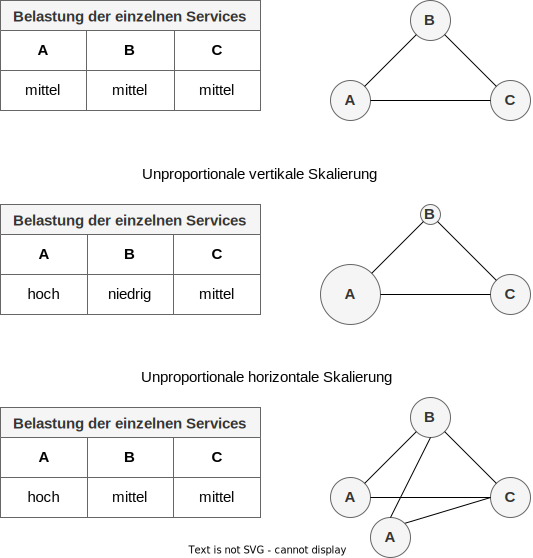
\includegraphics[width=0.8\textwidth]{images/scaling.pdf}
    \caption{Darstellung der beispielhaften Skalierungsmöglichkeiten eines Systems bestehend aus drei Services A, B und C, entsprechend bestimmter Lastszenarien}
    \label{fig:scaling}
  \end{figure}

\subsection{Aktualisierung}
\label{sec:update}
Wie bereits im Zusammenhang mit dem Entwicklungsprozess erläutert, bietet die lose Kopplung viele Möglichkeiten für die agile Weiterentwicklung eines serviceorientierten Systems. Einzelne Services können beispielsweise vollständig unabhängig voneinander weiterentwickelt und aktualisiert werden.\\
Daraus resultieren zumeist wesentlich frequentiertere Rollouts. Änderungen können auf Serviceebene ausgeliefert werden. Somit kann das Gesamtsystem kleinschrittig weiterentwickelt und aktualisiert werden, ohne dass jemals das komplette System neu aufgesetzt werden muss. Dabei ist zu beachten, dass dies nur möglich ist, wenn die Schnittstellen der einzelnen Services lediglich erweitert, nicht aber verändert oder verkleinert werden. Ansonsten kann es zu Inkompatibilitäten innerhalb des Gesamtsystems kommen. 

Im Folgenden werden nun drei Verteilungsstrategien für die Auslieferung von Aktualisierungen eines SOA Systems vorgestellt \cite{STORZ.2021}.

\textbf{Rollende Auslieferung}

Bei der rollenden Auslieferung von Services werden in einer geklusterten Umgebung nach und nach einzelne Hosts aus der Produktivumgebung genommen. Die neue Version wird auf dem Host eingerichtet. Anschließend wird der Host wieder in die Produktivumgebung eingepflegt. Dies ermöglicht die schrittweise Aktualisierung des gesamten Systems.\\
Der Vorteil ist, dass nicht direkt alle Instanzen aktualisiert werden, wodurch das Risiko im Fehlerfall begrenzt wird. Außerdem ist die Umsetzung der rollenden Auslieferung relativ einfach. Nachteil an dieser Verteilungsstrategie ist, dass einzelne Hosts zeitweise vom Netz genommen werden.\\
Abbildung \ref{fig:rolling} visualisiert den Ablauf einer rollenden Aktualisierung.\\

\begin{figure}[H]
  \centering
  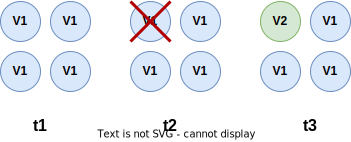
\includegraphics[width=0.5\textwidth]{images/rolling.pdf}
  \caption{Ablauf einer rollenden Aktualisierung}
  \label{fig:rolling}
\end{figure}

\textbf{Blue-Green Auslieferung}

Es wird parallel eine zweite Server-Instanz mit dem aktualisierten Service gestartet. Anschließend werden alle Nachrichten, die an den Service adressiert sind, über ein Lastenverteilungssystem an die aktualisierte Instanz geleitet. Im Falle eines Fehlers wird die Last wieder auf die alte Instanz geleitet. Tritt kein Fehler auf, so kann die alte Instanz heruntergefahren werden.\\
Vorteil dieser Strategie ist, dass praktisch keine Downtime auftritt. Außerdem kann ein Rollback relativ einfach realisiert werden, indem die Last wieder auf die alte Instanz geleitet und die aktualisierte Instanz wieder heruntergefahren wird.\\
Der Nachteil dieser Strategie ist, dass im Falle eines Fehlers 100 \% der Benutzer betroffen sind, bis der Fehler erkannt und die Last wieder auf die alte Instanz umgeleitet ist.\\
Abbildung \ref{fig:blue-green} visualisiert den Ablauf einer Blue-Green Aktualisierung.\\

\begin{figure}[H]
  \centering
  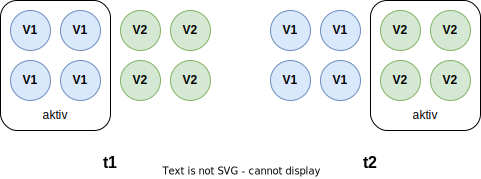
\includegraphics[width=0.7\textwidth]{images/blue-green.pdf}
  \caption{Ablauf einer Blue-Green Aktualisierung}
  \label{fig:blue-green}
\end{figure}

\textbf{Canary Auslieferung}

Die Canary Strategie ähnelt der Blue-Green Strategie, soll jedoch deren Probleme bei Auftreten eines Fehlers beheben. Sie kann angewendet werden, wenn jeweils mehrere Instanzen der zu aktualisierenden Services im System aktiv sind. Bei der Canary Strategie werden zunächst nur wenige aktualisierte Serviceinstanzen gestartet. Ein Teil der Anfragen werden anschließend über das Lastenverteilungssystem auf die neuen Instanzen geleitet. Treten bei der Benutzung keine Fehler auf, werden anschließend alle zu aktualisierenden Services im Blue-Green Verfahren ersetzt. Die Verwendung der Canary Strategie ist nur möglich, wenn gleichzeitig mehrere Versionen eines Services laufen können.\\
Vorteil dieser Strategie ist, dass im Fehlerfall nur eine Teilmenge der Benutzer betroffen ist. Außerdem gelten die gleichen Vorteile, die bereits bei der Blue-Green Strategie genannt wurden.\\
Der Nachteil dieser Strategie ist eindeutig die Komplexität in der Umsetzung. Die Verwendung der Canary Strategie ist nur zu empfehlen, wenn sie über ein Continuous Delivery (CD) System automatisiert ist.\\
Abbildung \ref{fig:canary} visualisiert den Ablauf einer Canary Aktualisierung.\\

\begin{figure}[H]
  \centering
  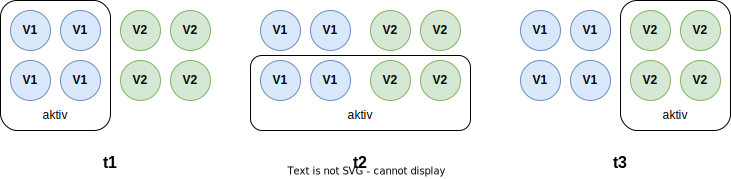
\includegraphics[width=\textwidth]{images/canary.pdf}
  \caption{Ablauf einer Canary Aktualisierung}
  \label{fig:canary}
\end{figure}


\subsection{Zusammenfassung der Auswirkungen}
\label{sec:deploymentSummary}
Es wurden unterschiedliche Aspekte der Auslieferung von serviceorientierten Systemen beleuchtet. Im Folgenden werden nun die konkreten Auswirkungen einer SOA auf den Auslieferungsprozess von Softwaresystemen zusammengefasst.

Zunächst ist die Einrichtung der einzelnen Services, unabhängig der Implementierungs-Technologie über das API der Virtualisierungs- oder Containersoftware ein wichtiger Punkt.\\
Virtualisierung wird zwar auch bei Systemen mit anderen Architekturen verwendet, ist aber zentral für SOA, da sie homogene Auslieferungs- und Installationsprozesse für heterogene Services ermöglicht.

Auch die verteilte Auslieferung der Systeme und die daraus resultierende erhöhte Komplexität des Auslieferungsprozesses ist eine zentrale Auswirkung der Verwendung einer SOA.\\
Alle Services des Systems müssen einzeln ausgeliefert werden und werden zudem üblicherweise auf unterschiedlichen Hosts eingerichtet. Dadurch wird der Auslieferungsprozess wesentlich komplexer als beispielsweise die Auslieferung eines monolithischen Systems.\\
Um diese Komplexität zu verringern, wird zunehmend \textit{serverlos} ausgeliefert. Dabei wird der Code der Services an einen Anbieter für serverlose Auslieferung weitergegeben, welcher dann beliebig viele Instanzen in gewünschter Konfiguration auf eigener Infrastruktur ausliefert. Dabei übernimmt dieser Anbieter die gesamte Verwaltung der Infrastruktur und stellt die Funktionalität der Services über ein Netzwerk bereit. Die Verwendung einer serverlosen Auslieferung hat den Vorteil, dass der Auslieferungsprozess erheblich vereinfacht wird und keine eigenen Hosts mehr verwaltet werden müssen. Im Austausch mit diesen Vorteilen stehen die Vertrauenswürdigkeit der Anbieter und die Tatsache, dass der Herausgeber der Services keinerlei Kontrolle darüber hat, wo diese laufen \cite{STORZ.2021}.

Auch die Auswirkungen auf die Skalierung eines Systems wurden bereits beschrieben. Bei der Auslieferung von monolithischen Systemen wird beispielsweise eine Instanz des Systems auf einem Host eingerichtet. Um diese Systeme skalieren zu können, wird je nach Art des Systems entweder die bestehende Instanz auf einen leistungsfähigeren Host verschoben oder es werden weitere Instanzen des Systems auf anderen Hosts aufgesetzt, die sich die vorhandene Last anschließend teilen.\\
Bei serviceorientierten Systemen werden die einzelnen Services hingegen einzeln ausgeliefert und skaliert.\\
Für die flexible Skalierbarkeit der Systeme und dem damit einhergehenden \textit{deployment on demand} wird eine Art Service Provider benötigt, der bei Bedarf weitere oder leistungsfähigere Serviceinstanzen bereitstellen und ausliefern kann \cite{NADAREISHVILI.2016}. Diese Möglichkeiten führen zu deutlich erhöhter Komplexität der Infrastruktur, wenngleich sie enorme Vorteile für die Flexibilität eines Systems bieten.

Eine weitere Auswirkung der SOA auf den Auslieferungsprozess sind wesentlich kleinschrittigere Aktualisierungen und daraus resultierend wesentlich frequentiertere Auslieferungen ohne Downtime des Systems (beispielsweise durch Blue-Green oder Canary Auslieferung).

Insgesamt ist also erkennbar, dass die Verwendung einer SOA zu einem komplexeren Auslieferungsprozess führt. Um diese Komplexität handhabbar zu machen, werden zumeist umfangreiche DevOps Systeme für die Unterstützung im Entwicklungs- und Auslieferungsprozess verwendet.\\
Diese führen bei zielgerichteter Benutzung zu einer besseren Organisation, die sich bereits im Entwicklungsprozess positiv auswirkt. So ist beispielsweise eine gut organisierte Quellcodeverwaltung eine essenzielle Basis, um die isolierte Entwicklung homogener Services gut strukturiert durchführen zu können und aus diesen zu einem späteren Zeitpunkt komplexe Systeme zusammensetzen zu können. Darüber hinaus unterstützen diese Systeme das Konfigurations- und Releasemanagement, um die Zusammensetzung, Parametrisierung und Versionierung der serviceorientierten Softwarelösungen zu automatisieren. Dies reduziert Fehler und Inkonsistenzen, sowohl im Stadium der Entwicklung, als auch im Auslieferungsprozess. Eine gute Organisation und konsistente Daten sind beispielsweise auch nötig, um Systeme für Wartungsarbeiten, Recovery- und Testszenarien reproduzierbar zu machen.\\
In vielen DevOps Systemen lassen sich außerdem sogenannte \textit{Pipelines} einrichten, über welche umfangreiche Ausführungsfolgen automatisiert werden können. Eine solche Pipeline kann zum Beispiel nach Fertigstellung einer Aktualisierung automatisiert gestartet werden. Im Durchlauf der Pipeline werden dann beispielsweise die Paketierung und Einrichtung der Software in einer VM angestoßen werden und der aktualisierten Service wird als VM-Image für den Kunden bereitgestellt oder direkt auf dessen Zielhosts ausgerollt.

Die Möglichkeit, Systeme in Form von einzelnen Services auszuliefern und dadurch unabhängig voneinander erweitern, skalieren und aktualisieren zu können, birgt je nach Anwendungsfall also enorme Vorteile, führt im gleichen Zug jedoch auch zu erheblicher Steigerung der Komplexität bei der Auslieferung. Diese Komplexität kann durch geeignete Hilfssysteme zwar wieder reduziert werden, dies ist jedoch mit sehr hohem initialen Aufwand verbunden.\\
Die Verwendung einer SOA lohnt sich hinsichtlich der Auswirkungen auf den Auslieferungsprozess also nur, wenn die dadurch gewonnenen Vorteile auch ausgeschöpft werden.